\documentclass[a4paper, 12pt, onecolumn]{article} 

% To change the distance between the columns when using `twocolumn`:
\setlength{\columnsep}{0.5in} % Source: tex.stackexchange.com/a/24563/110560


%% Read https://texblog.org/2012/08/29/changing-the-font-size-in-latex/ for reference on font sizes.

% For margins. 
% Source: kb.mit.edu/confluence/pages/viewpage.action?pageId=3907057. 
% Also see: https://www.sharelatex.com/learn/Page_size_and_margins
\usepackage[margin=1.0in]{geometry}  

 % For the "comment" environment to make LaTeX comments
\usepackage{verbatim} 

% For equations \begin{equation*}:
\usepackage{amsmath, amssymb}  

% For tables using \begin{longtabu}:
\usepackage{tabu, ltxtable, tabularx, longtable}

% For captions on longtabu, see tex.stackexchange.com/q/268927/110560
\usepackage{caption}
\captionsetup[longtable]{skip=9pt, margin=0.1\textwidth,
	 justification=justified, singlelinecheck=false}	% Source: tex.stackexchange.com/a/95208/110560 and tex.stackexchange.com/a/3178/110560 and tex.stackexchange.com/a/88817/110560 and tex.stackexchange.com/a/37793/110560

% For images using \begin{figure} and for \scalebox{}:
\usepackage{graphicx}
\graphicspath{Images/}  % Location of the graphics files (set up for graphics to be in PDF format)

% For using bullets in description lists.
\usepackage{enumitem}

% For Neural Network Diagrams, see http://tex.stackexchange.com/a/132471/110560
\usepackage{tikz}
\usetikzlibrary{matrix,chains,positioning,decorations.pathreplacing,arrows}


\addtolength{\footnotesep}{1mm} % Source: tex.stackexchange.com/a/141938/110560.

% For URLs with \url{blahblahblah}
\usepackage{url} % Source: http://tex.stackexchange.com/a/40222/110560

% For rotating figures with \begin{sidewaysfigure}
\usepackage{rotating}

\begin{document}
	
	

%\hspace{5em} Normalization:
%\begin{equation*}
%x_{i, 0...1} = 
%\frac	{ x_{i} - x_{min}	}
%{ x_{max} - x_{min}	}
%\end{equation*}

	
%% NSL Test Set with SMOTE and Random Undersampling:
%\centering \begin{longtabu} to \textwidth {| l | c | c | c | c | } \hline
%	& Precision & Recall	& F1 score  & Support	\\ \hline
%	DoS   	& 93\%   	& 84\%      & 88\%      & 7457		\\ \hline
%	Normal	& 73\%   	& 95\%      & 83\%      & 9710		\\ \hline
%	Probe 	& 64\%   	& 57\%      & 60\%      & 2421		\\ \hline
%	R2L   	& 64\%   	& 12\%      & 20\%      & 2754		\\ \hline
%	U2R 	&  5\%     	& 16\%      & 8\%       & 200		\\ \hline
%	Total 	&  76\%     & 76\%   	& 76\%   	& 22542		\\ \hline
%	\caption{Decision Tree on NSL Test Set with SMOTE and Random Undersampling. Total Accuracy = 76.32\%}
%\end{longtabu}


%\begin{figure}[!h]
%	\centerline{}
%	\caption{An Artificial Neural Network with one hidden layer, working on a dataset with three predictors and two target classes.}
%	\label{fig: ANN}
%\end{figure}


%\input{"Sections/Notation and nomenclature"}
%\input{"Sections/The goal of Backpropagation"}
%\input{"Sections/Forward pass"}


%\scalebox{1.7}{
	%{}^{14}\text{C}^{15}	%% Source: tex.stackexchange.com/a/30563/110560
	
%}

%\input{"Diagrams/Generic Neuron"}
%\\
%\centering Generic Neuron
%\input{"Diagrams/Example Network"}


\title{Mobile-controlled wireless rover with IR sensors}

\author{
	Abhishek Divekar (131080051) \\ 
	Vaibahav Savla (131080051) \\ 
	Meet Parekh (131080051) \\ 
	\\
	Veermata Jijabai Technological Institute\\
	H. R. Mahajani Marg, Matunga, Mumbai - 400031,\\ 
	Maharashtra, India\\
}

\date{}	%Source: tex.stackexchange.com/a/2761/110560

\maketitle

\thispagestyle{empty}

\begin{abstract}
	Wireless, sensor-driven robotics is a discipline with ready applications in military, factory and civilian uses. While they initially lacked robustness due to the inherent problems associated with wireless technology such as fluctuating signal strength and difficulty in debugging, the technology has now matured such that several critical services and mechanisms now operate wirelessly. Coupled with the ubiquity of Wireless LAN technology and the Internet, we find that there are some interesting use cases for remotely-controllable vehicles. 
	
	In this paper we both provide the specifications for and build a movable robot which may be controlled from any device connected to the same Wireless LAN, via a Web 2.0 interface. IR sensors feed information back to the controlling human, allowing them to maneuver accordingly based on the terrian.
	
	While not suitable for industry or military grade applications, this setup was found to be robust from an experimental and academic viewpoint.
\end{abstract}



\section{Introduction}

\begin{description}[font=\quad $\circ$, topsep=-2pt, itemsep=2pt]
	\item Rovers have been widely employed by military and research community (space research) to explore unknown terrains. However rovers have also been in use for simpler applications such as monitoring of different zones on the factory floor. Be it simple or complex rover, they present two major challenges:
	
	\begin{enumerate}[itemsep=0em]
		\item Interaction with the environment
		\item Wireless control
	\end{enumerate}
	
	\item In comparison with the scientific Mars rovers which are voluminous beasts of the order of a few hundred kilograms \cite{RobotSizes}, our rover is a simple three-wheeled bot weighing slightly more than a 1500 grams. The motors power the back wheels and the front wheel is simply a ball-bearing with a low coefficient of friction, allowing the rover to move quickly over smooth surfaces.

	\clearpage
	\quad A block-diagram of the overall hardware system is as follows:

	\begin{figure}[ht]	% Source: http://tex.stackexchange.com/q/131259/110560
		\centering
		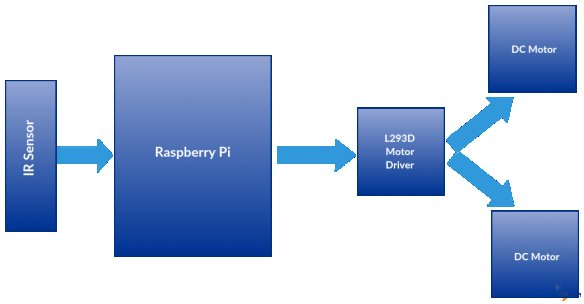
\includegraphics[width=\linewidth]{"./system_diagram.jpg"}
		\caption{System diagram of the rover}
		\label{fig:System Diagram}
	\end{figure}

	\item The microcontroller used is the Raspberry Pi 3, a popular and well-supported hobbyist board. It comes bundled with an onboard Wireless chip and 40 General Purpose Input/Output pins for interfacing with the motors and IR sensors. Power is supplied via a pair of 9v batteries (to the motors) and a 5600 mAh powerbank (to the Pi). The controlling GUI is served by a Python Django server running on Raspbian, a Linux-based distribution installed on the Raspberry Pi’s external memory.

	\item The DC motors that move the rover around are standard 300 rpm high-torque motors \cite{300RPMMotors} (low torque motors were unsuccessful in moving the rover on even flat surfaces). The power is delivered via 9v batteries, and controlled via a L293D motor driver. 


	\item An important module of the rover is the trio of IR sensors on the bottom panel, around one inch above the ground. They are used to detect the terrain (black or white) and can be used for line-following even in dim environment. While sufficient for our current purposes, it is possible to replace them with complex, application-specific sensors if required e.g. landmine-detection apparatus for military use cases. \\

	\begin{figure}[ht]	% Source: http://tex.stackexchange.com/q/131259/110560
		\centering
		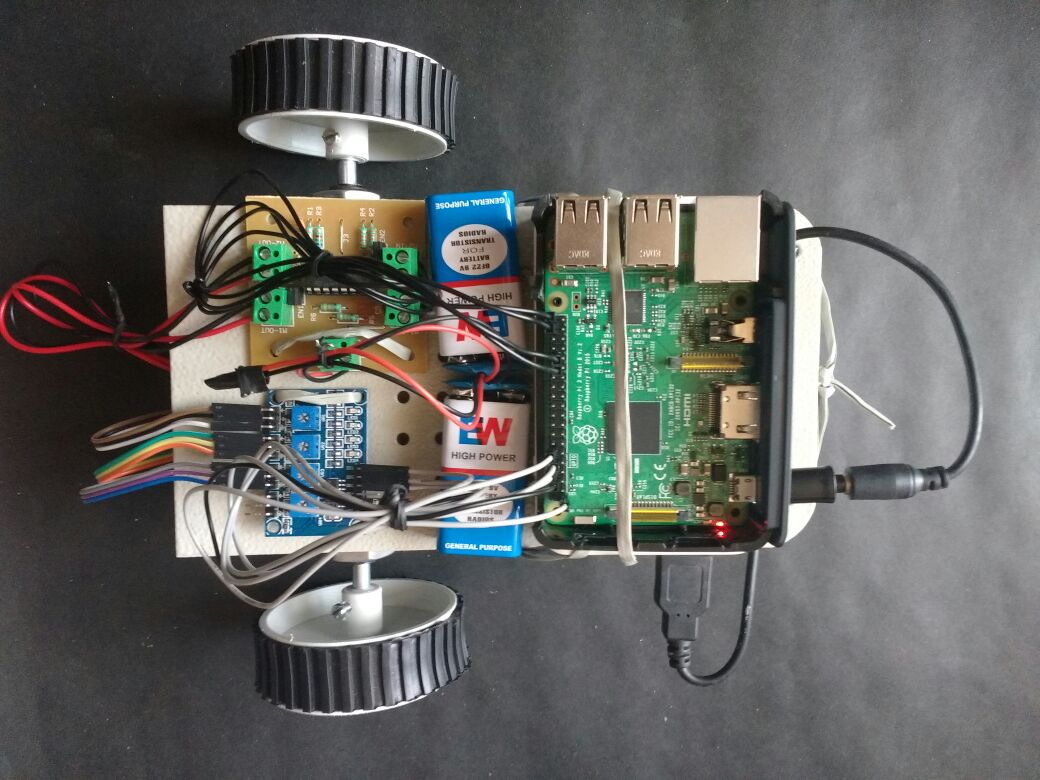
\includegraphics[width=\linewidth]{"./bot-pic-top.jpg"}
		\caption{A photograph of the assembled rover}
		\label{fig:BotPicTop}
	\end{figure}
	
\end{description}

While not nearly state-of-the-art, this setup is sufficient for the proof-of-concept which we build.



\clearpage


\section{Motivation}


\quad \quad The main aim of the project is to learn about embedded systems as a whole, and along the way display the applicability and robustness of wireless technology in robotics. We do so using a movable, proof-of-concept rover which we then control using a GUI interface accessible through either a mobile phone or laptop, anywhere in the vicinity. A simple extension of this notion would allow the control of robots in other countries or even on other planets. 


\section{Problem Definition}

\begin{enumerate}
	\item To construct a movable robot, with a 15x8 chassis, two wheels and three IR sensors attached to a makeshift cardboard bottom, and a Raspberry Pi 3B and DSG powerbank secured to the top. The IR sensor board and motor drivers are secured to the chassis with electrical tape or plastic cords to prevent movement.
	
	\item The Raspberry Pi automatically connects to a known Wireless LAN at bootup, thus allowing unsupervised bootups at regular intervals.
	
	\item A Web 2.0 interface would be served via a Python Django server to a computer ${}^{\ref{WhatsAComputer}}$ connected to the same Wifi network as the Pi. This interface serves the controls \textit{"Forwards"}, \textit{"Backwards"}, \textit{"Left"}, \textit{"Right"} and \textit{"Stop"}. The interface is served at an IP address known to the computer, removing the problem of reconfiguration. 

	\footnotetext[1]{\label{WhatsAComputer} Note that our only criterion for \textit{computer} is a device with a JavaScript-enabled web browser that is able to communicate via HTTP requests. We may thus use mobile phones (Android, iOS etc.) or laptop or desktop computers to access this interface.}	% Source for footnotes: latex-tutorial.com/tutorials/beginners/07b-footnotes/
	
	\item The interface would additionally display the status of three IR sensors as binary values, e.g. $010$, indicating the middle senor was triggered. This would be updated every few seconds without reloading the page. This is for reference of the human controller, similar to a video feed (which was infeasible due to bandwidth constraints).
	
	\item On clicking one of the buttons, a request would be sent over the Wireless connection to the Django server, which would in turn send a message to the motor drivers, moving the rover in the desired direction (or stopping it). 

\end{enumerate}

Note that this is a proof-of-concept project. Every stage would require changes in hardware materials and electronics to build a workable rover system.



\clearpage

\input{"Methodology and Implementation"}



\clearpage

\begin{thebibliography}{10}	%% Source: met.guc.edu.eg/OnlineTutorials/LaTeX/Bibliographies%20and%20Citation.aspx
	
	\bibitem{RobotSizes} NASA, \textit{Mars Science Laboratory Landing}, pg 34: \\
	\url{https://www.jpl.nasa.gov/news/press_kits/MSLLanding.pdf}
	
	
	\bibitem{Pi3BPinDiagram} Raspberry Pi 3B pin diagram: \\
	\url{http://pi4j.com/pins/model-3b-rev1.html}

	
	\bibitem{300RPMMotors} 300 RPM motors specification: \\
	\url{http://robokits.co.in/motors/high-torque-dc-geared-motor-300rpm}
	
	\bibitem{L293D_MotorDriver} L293D motor driver specification: \\
	\url{https://www.engineersgarage.com/sites/default/files/L293D.pdf}
	

	\bibitem{RPi3BSpecs} Raspberry Bi 3 Model B specifications: \\
	\url{https://www.raspberrypi.org/documentation/hardware/computemodule/RPI-CM-DATASHEET-V1_0.pdf}
		
	
	
	
	\bibitem{latexMath} Graetzer George, \emph{Math Into \LaTeX},
	Birkhäuser Boston; 3 edition (June 22, 2000).
	
\end{thebibliography}

\end{document}  % The End